% Report skeleton (Point 11a): IEEE conference template, guideline section order,
% about 8 pages plus references. Edit here or on Overleaf (upload this folder and
% results/figures/). Every figure and table comes from the results files written
% by the experiment commands in the README, so the numbers always match the code.
% Lines starting with "TODO" are notes for the author; remove them before submission.
\documentclass[conference]{IEEEtran}
\usepackage{graphicx}
\usepackage{booktabs}
\usepackage{amsmath}
\usepackage{cite}
\graphicspath{{../results/figures/}{figures/}}

\begin{document}

\title{Should the Robot Trust Its Map?\\Learning Calibrated Trust in Unreliable Semantic Priors}

\author{\IEEEauthorblockN{Khaled Obeid}
\IEEEauthorblockA{COE750, Lebanese American University}}

\maketitle

\begin{abstract}
% TODO: about 150 words: problem, two-dial world, PPO with masking against an exact optimum, main findings (H1-H4).
\end{abstract}

\section{Introduction}
% TODO: semantic prior maps can be wrong and their confidence can lie; motivation from
% confidence-weighted semantic maps (thesis link is motivation, not a contribution, 10b).
% State the research question (Point 1) and the three contributions C1-C3 (10b).

\section{Background}
% TODO: MDPs and value iteration (exact optimum over current room x searched set, 160 states);
% Q-learning (E0); PPO \cite{schulman2017ppo} with GAE \cite{schulman2016gae} and action masking \cite{huang2022closer}.

\section{Related Work}
% TODO: at least 10 papers from 2024--2026; closest work \cite{castelobranco2026};
% overconfidence in semantic mapping \cite{marques2024overconfidence,prasanna2024perception}.

\section{Methodology}
\subsection{World and episodes}
% TODO: generated houses (Point 3a, \cite{deitke2022procthor,lopes2010constrained}), co-occurrence table (3b),
% claim, reliability r ~ Beta(10(1-rho), 10 rho), displayed confidence c = sigma(kappa logit r), lambda mixture (3c).
\subsection{Observation, actions and reward}
% TODO: 5 shuffled rows x 5 features (4a), variant masks (4c), masked room choice (5a),
% reward in house-widths with the 3-decision cap and failure penalty 1, gamma = 1 (Point 6).
\subsection{Learning agents and baselines}
% TODO: MaskablePPO, 64-64 tanh, settings of 7c \cite{raffin2021sb3}; exact optimum with true r (8a);
% regret (8b); baselines (8d).

\section{Experimental Setup}
% TODO: training rho ~ U[0, 0.8] (9a), 1M decisions (a run stops at 1,015,808, 62 rollouts),
% validation every 50k on 1,000 episodes, 5 seeds per main variant (7d);
% test set 5,000 episodes per rho, 25 per test house (9b); 95% t-intervals over seeds \cite{agarwal2021precipice}.

\section{Results}
\subsection{E0: tabular Q-learning reaches the optimum}
\begin{figure}[t]\centering
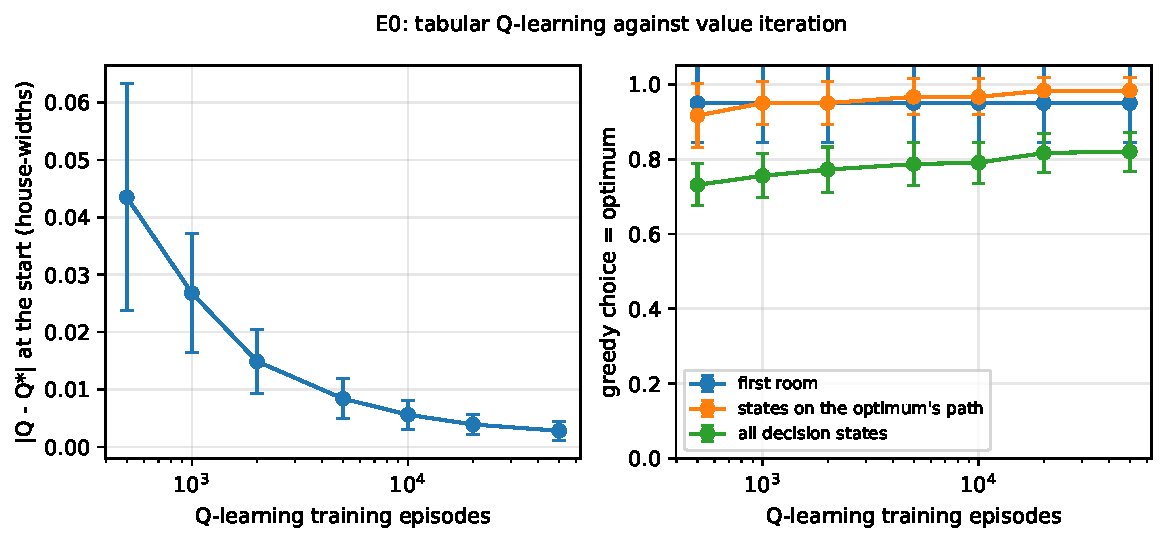
\includegraphics[width=\columnwidth]{e0_qlearning}
\caption{E0. TODO caption (results/e0/curve.csv).}\label{fig:e0}
\end{figure}

\subsection{E1: when does the map stop being worth following? (H1)}
\begin{figure*}[t]\centering
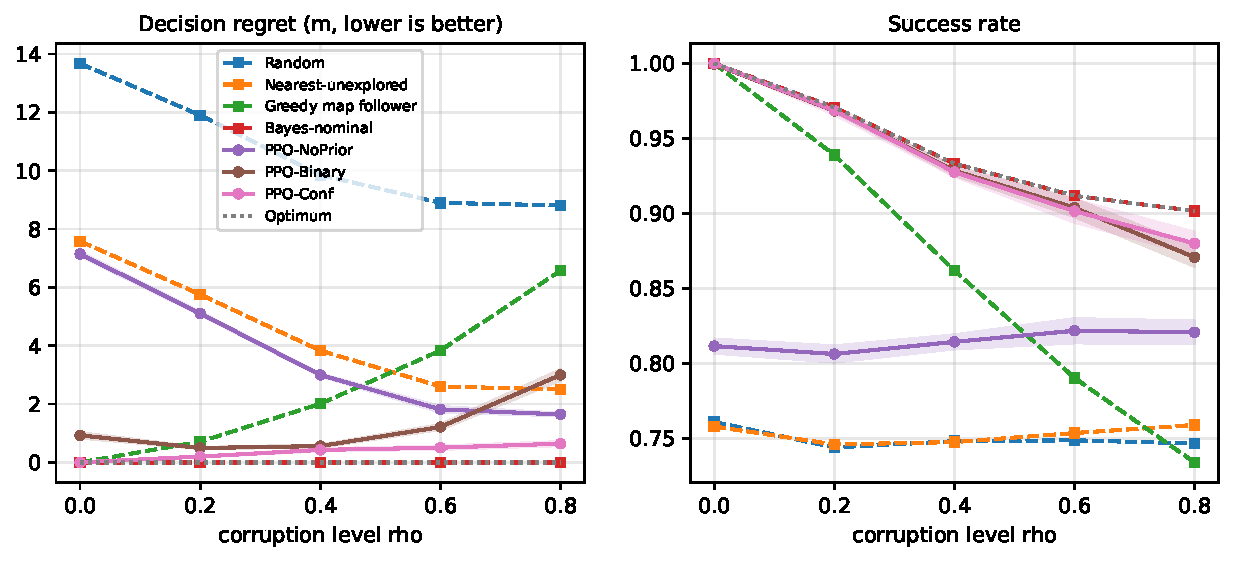
\includegraphics[width=0.85\textwidth]{e1_regret}
\caption{E1. TODO caption (results/e1/table.csv).}\label{fig:e1}
\end{figure*}

\subsection{E2: does trust switch at c*? (H2)}
\begin{figure*}[t]\centering
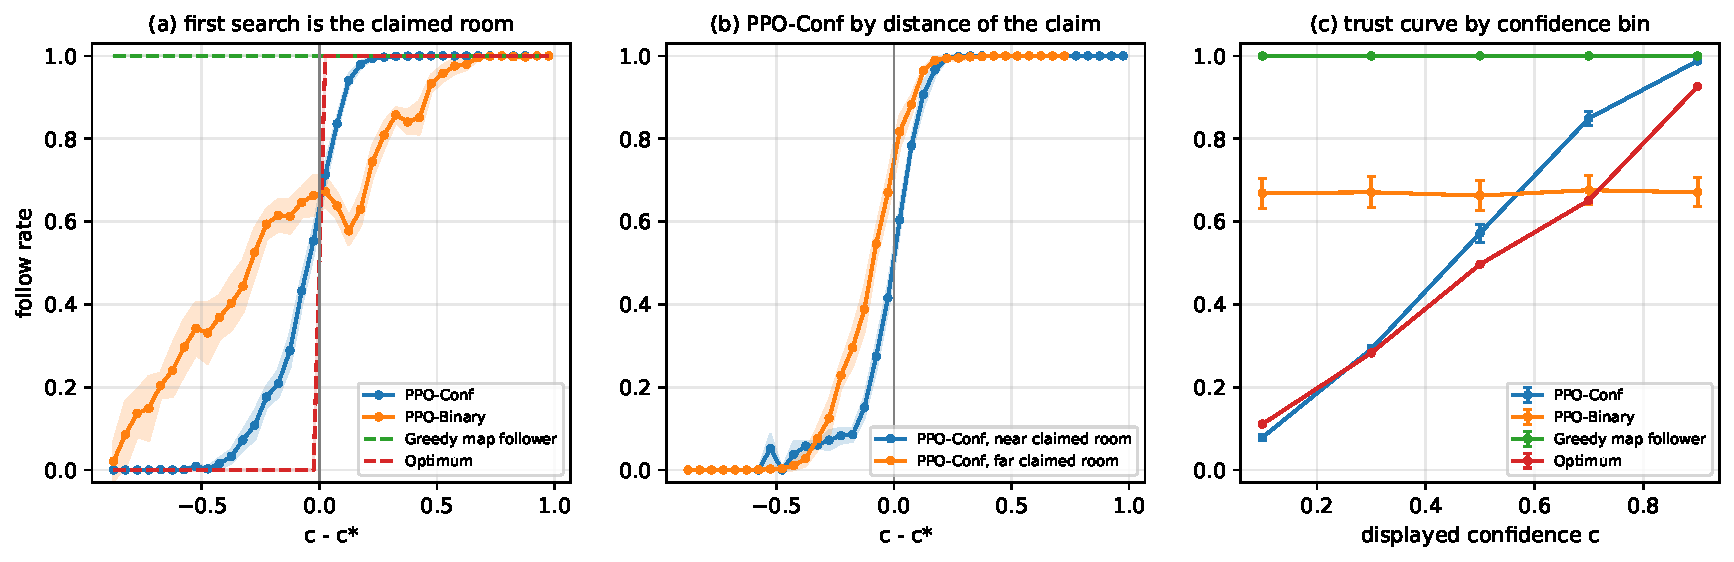
\includegraphics[width=\textwidth]{e2_trust}
\caption{E2. TODO caption (results/e2/follow.csv).}\label{fig:e2}
\end{figure*}

\subsection{Value of the map by habit strength (H4)}
\begin{figure}[t]\centering
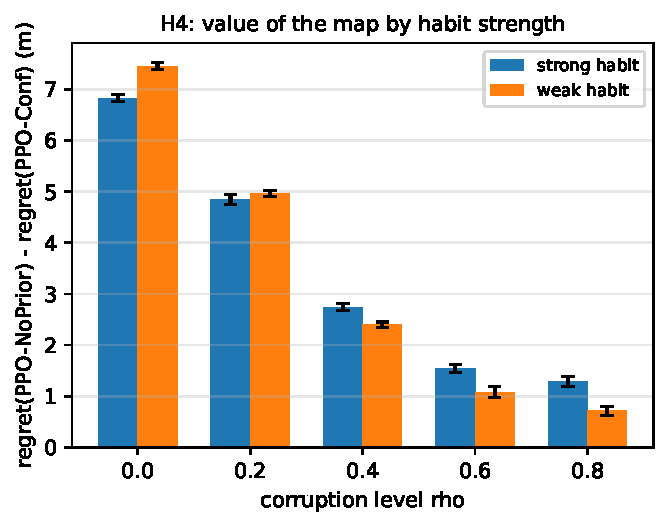
\includegraphics[width=\columnwidth]{h4_habit_gap}
\caption{H4. TODO caption (results/e1/h4.csv).}\label{fig:h4}
\end{figure}

\subsection{E3: calibration (H3)}
\begin{figure*}[t]\centering
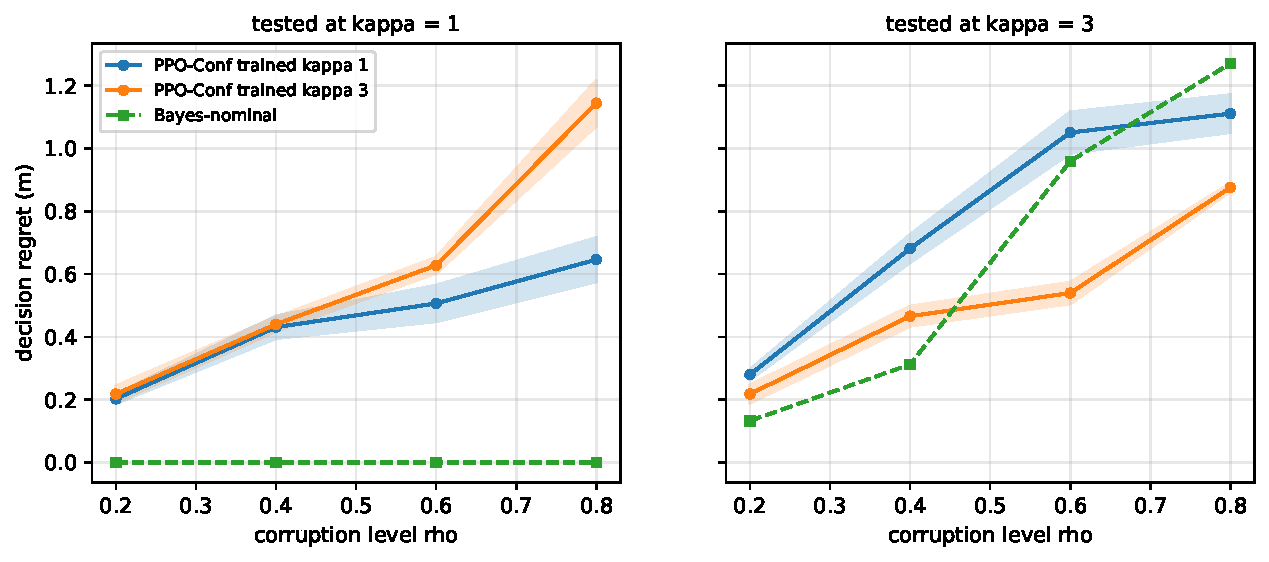
\includegraphics[width=0.85\textwidth]{e3_calibration}
\caption{E3. TODO caption (results/e3/table.csv).}\label{fig:e3}
\end{figure*}

\subsection{Gazebo evaluation}
% TODO: two rows (Cost of a decision): decision metrics on planned distance (equal to 2D),
% end-to-end metrics (driven distance, overhead, Nav2 failure rate); results/gazebo/.

\section{Discussion}
% TODO: limitations: the error model (Beta, lambda, table) is ours; PPO-Binary's crossover depends on the
% training mix (9a); first-decision success and on-the-way searches (Q8); future work.

\section{Conclusion}
% TODO

\section*{Contribution Statement}
This is a solo project; all design choices, implementation, experiments and writing are the work of Khaled Obeid.

\section*{Acknowledgment}
This work uses Stable-Baselines3 and sb3-contrib, Gymnasium, ROS~2, Nav2 and Gazebo. Claude (Anthropic) was used
as a design-discussion partner and coding assistant; the author is responsible for every choice and result.

\bibliographystyle{IEEEtran}
\bibliography{refs}

\end{document}
